\chapter{Análise dos Resultados}
\label{cap:04}
Neste capítulo, são apresentados e discutidos os resultados obtidos na aplicação dos métodos de segmentação de imagens propostos neste trabalho, com ênfase nas imagens de média e baixa resolução. Utilizando o modelo Segment Anything (SAM), avaliou-se a eficácia do método utilizado, que utilize inteligencia artificial para aprimorar a precisão da segmentação.

Para uma análise quantitativa robusta, foram adotadas as métricas Mean Squared Error (MSE) e Normalized Cross-Correlation (NCC), além de um método específico criado para complementar a avaliação dos segmentos. Estes indicadores foram aplicados para avaliar a qualidade das segmentações produzidas, comparando-as com padrões de segmentação existentes. Este capítulo tem, portanto, como objetivo apresentar as análises qualitativas e quantitativas dos resultados, destacando os avanços e as limitações do método proposto em relação aos métodos tradicionais.

\section{Desenvolvimento do sistema}

Nesta seção será apresentado todos os processos em python realizados para a criação do código de análise dos dados criados e os já existentes realizados pelo autor, o desenvolvimento foi iniciado com a implementação das mascaras geradas pelo segment anything como mostra a Figura \ref{fig:code1}.

\FloatBarrier
\begin{figure}[ht]
    \caption{Código utilizando o SAM para retornar a segmentação}
    \centering
    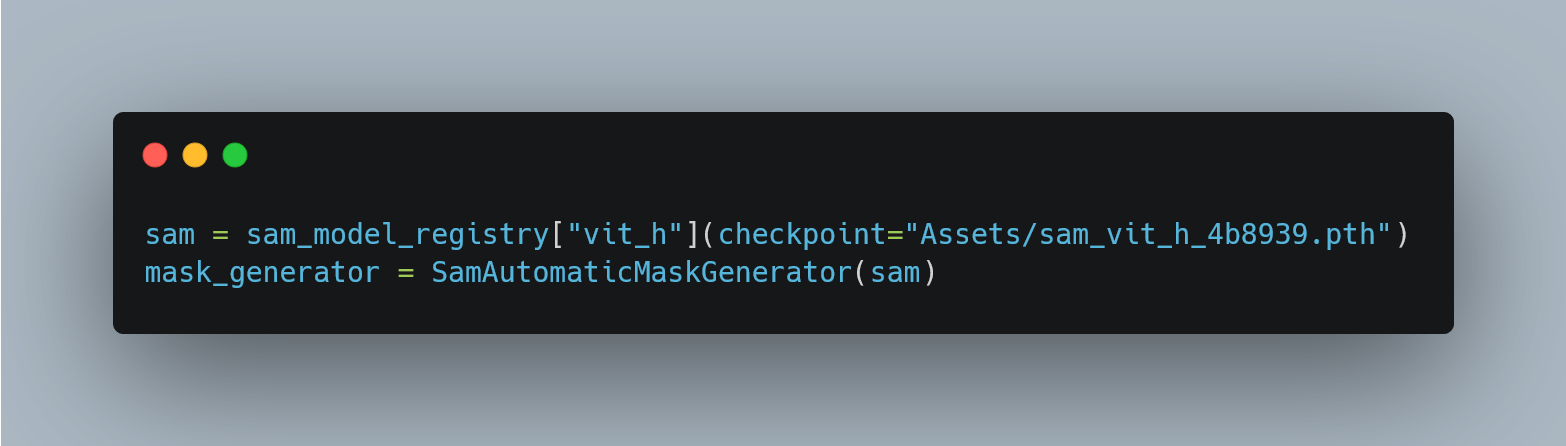
\includegraphics[scale=0.25]{imagens/code_part_one.png}
    \label{fig:code1}
\end{figure}
\FloatBarrier

Nesse processo a função faz o acesso do modelo que no caso utilizado foi o model vit h pesando 2.38 Gigabytes de memória, para essa função é possível a utilização de dois caminhos de processamento da imagem atual, o primeiro deles é utilizando a GPU de uma placa de vídeo o que em tese poderia diminuir o gargalo gerado nas CPUs e melhorar a velocidade em que é executado, logo após a geração das mascaras pelo SAM, o próximo passo é justamente iniciar a criação das mascaras manualmente.


Para essa etapa foi utilizado várias pixel artes retiradas do site: itch.io que tem grande parte da comunidade servindo \textit{assets} gratuitos para projetos pessoais ou jogos \textit{indie}, a execução dito foi realizada com uma visão humana para servir de referencia para os resultados gerados da inteligencia artificial, mas para as respostas do SAM não temos a geração de uma imagem em si mas de um \textit{array} de camadas criadas com cada segmento gerado, para isso se tornar uma imagem é necessário este código mostrado na Figura \ref{fig:code2}.

\FloatBarrier
\begin{figure}[ht]
    \caption{Código para o método próprio de análise}
    \centering
    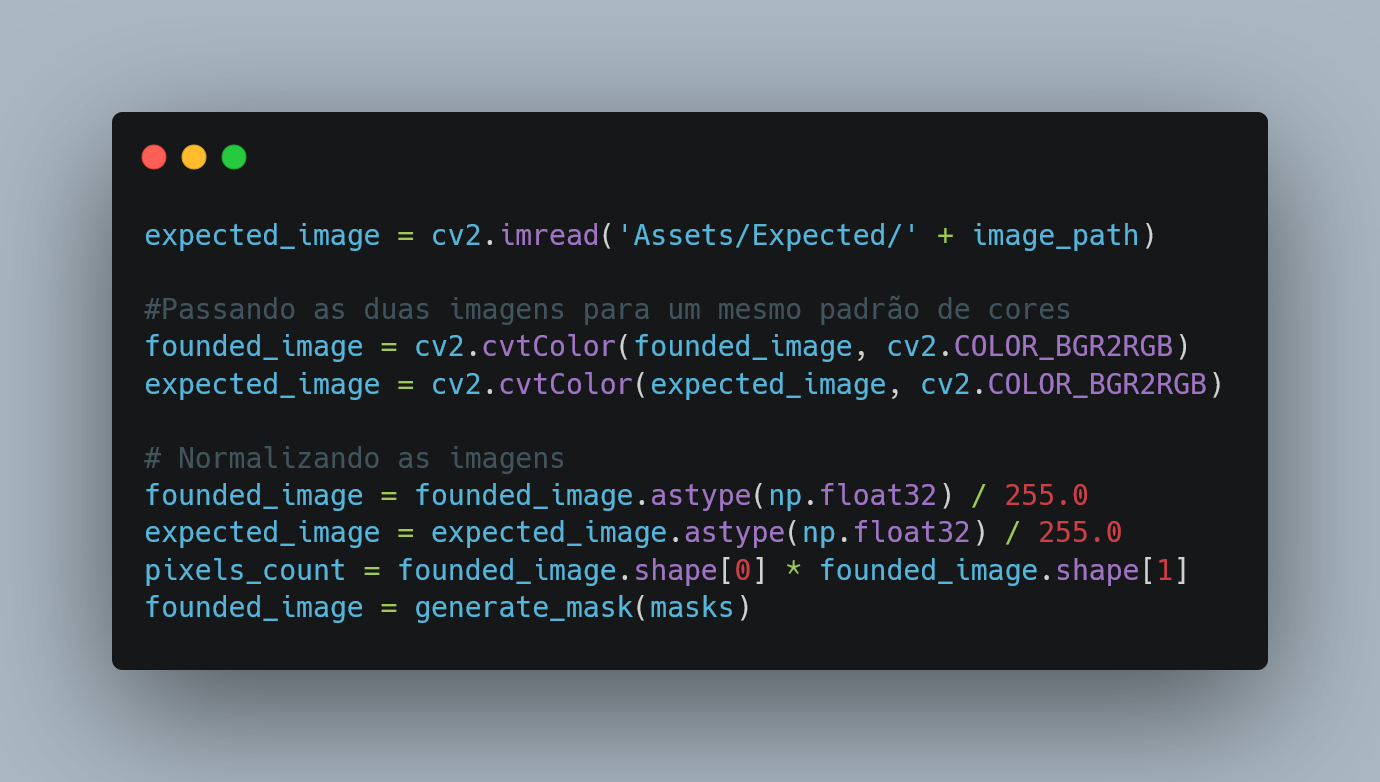
\includegraphics[scale=0.25]{imagens/code_part_two.png}
    \label{fig:code2}
\end{figure}
\FloatBarrier

Após os dois tipos de imagem já estarem preparados para a comparação é necessário a utilização de mais de um método de análise para compararmos e abrangermos mais pontos em comum sobre o resultado esperado, por isso é utilizado neste momento três tipos de análises, sendo duas delas configuradas pela biblioteca Scikit, a outra foi realizada pelo autor com a tentativa de gerar resultados diferentes dos métodos padrões.

O processo foi desenvolvido analisando a imagem pixel a pixel, começando no canto superior esquerdo, o primeiro pixel (coordenada zero). A varredura percorre cada linha da esquerda para a direita e, ao final de cada linha, passa para a próxima. Cada pixel possui duas referências: uma para a imagem original, segmentada pelo autor, e outra para a segmentação feita pela inteligência artificial (IA). Para cada pixel na imagem original, cria-se uma conexão com o pixel correspondente na imagem gerada pela IA, e o processo continua até que uma diferença de cor seja detectada entre os pixels correspondentes das duas imagens. Quando isso ocorre, o código verifica qual imagem apresentou a diferença primeiro; se a diferença for detectada primeiro na imagem original, o código marca essa mudança no grupo segmentado criando assim o inicio de uma nova conexão entre os pixels, mas, se a diferença aparecer apenas na imagem da IA, o pixel é marcado como incorreto, indicando um possível erro da IA, pois a imagem original ainda mantém a mesma cor. Ao final, a análise calcula a porcentagem de erros comparando o número de pixels incorretos com o total de pixels da imagem, todo este processo é feito nessa função do código-fonte como mostra a Figura \ref{fig:code3}.

\FloatBarrier
\begin{figure}[ht]
    \caption{Código para receber os valores de cada tipo de análise}
    \centering
    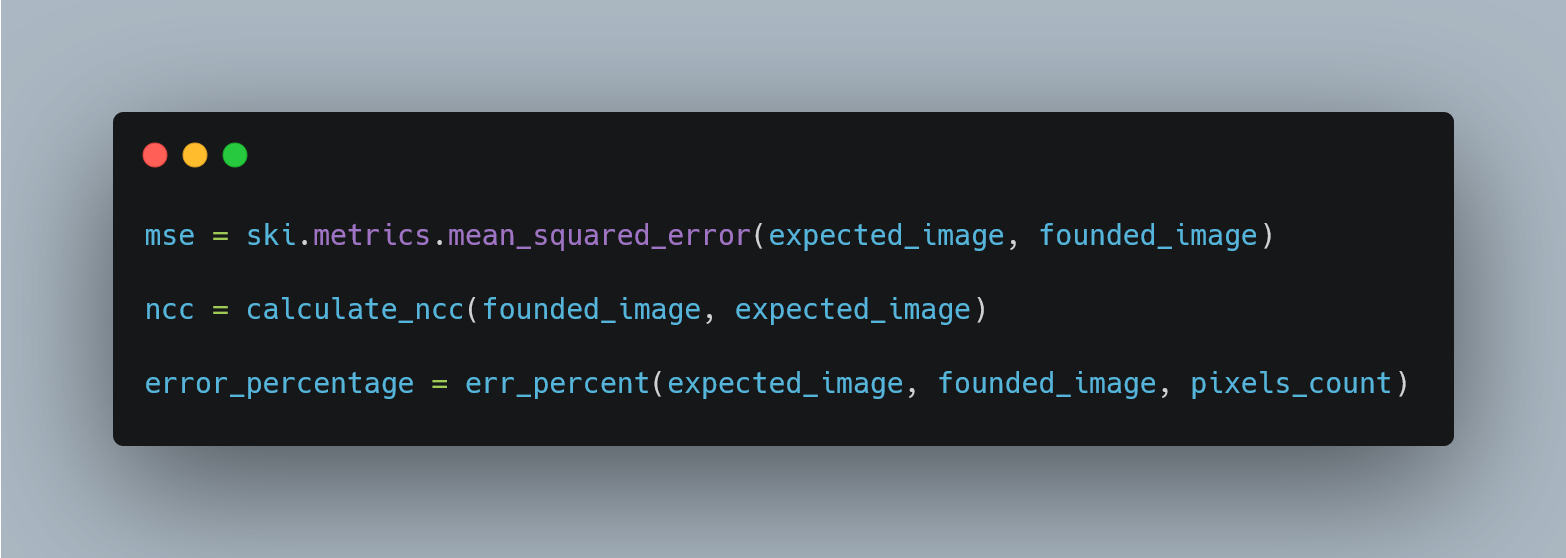
\includegraphics[scale=0.25]{imagens/code_part_three.png}
    \label{fig:code3}
\end{figure}
\FloatBarrier

Além da análise própria, também foram utilizados o método NCC e o MSE, que serão abordados a seguir. O primeiro deles, o NCC (Normalized Cross Correlation), é uma técnica usada para medir a similaridade entre imagens. Nela, utiliza-se geralmente uma imagem de referência e uma imagem-alvo; o índice de correlação varia de -1 a 1, onde valores mais próximos de 1 indicam alta similaridade, valores próximos de zero indicam baixa ou nenhuma correlação com a imagem de referência, e o valor -1 representa uma correlação inversa com a imagem. No entanto, o NCC não é vantajoso para casos em que há imagens complexas para analisar, o que é o oposto das imagens-alvo deste estudo.

O segundo método, o MSE (\textit{Mean Squared Error}), é uma técnica utilizada para avaliar a diferença entre duas imagens ao medir o erro médio entre os pixels correspondentes. O MSE calcula a média dos quadrados das diferenças de intensidade entre os pixels das duas imagens, gerando um valor que representa o grau de discrepância entre elas. Quanto maior o valor do MSE, maior a diferença entre as imagens comparadas; valores próximos de zero indicam alta similaridade. Esse método é simples e eficaz para medir discrepâncias, mas pode ser sensível a pequenas variações de pixel, sendo ideal para imagens onde os detalhes e as variações sutis são relevantes.

A combinação dessas três análises permite uma avaliação mais completa e detalhada da similaridade e discrepância entre as imagens, onde cada método contribui com uma perspectiva distinta. O cruzamento dos resultados oferece um panorama mais robusto, permitindo identificar falhas localizadas, medir a correlação global e quantificar as diferenças de intensidade de forma precisa. Essa integração facilita a obtenção de dados mais confiáveis e detalhados sobre o desempenho da segmentação, ampliando a compreensão sobre as sutilezas entre as imagens e fortalecendo a precisão das conclusões finais.

\section{Agilidade e Eficiência}
Nessa seção será abordado o fator velocidade para o processo ser finalizado, ou seja, independente dos resultados qual a margem de tempo destinada apenas a realização da segmentação das imagens, lembrando que isso seria apenas um fragmento de todo o desenvolvimento da ferramenta.

Como o esperado, foi identificado nos computadores usados para executar o código uma quantidade de tempo razoável até sua finalização,apesar disso, entre eles houveram minímas diferenças de tempo de execução, mesmo com abruptas diferenças de processamento, em seguida será mostrado as propriedades de cada um deles, para uma melhor comparação da média dos resultados obtidos em termos de desempenho, como mostra a Tabela \ref{tab:comparacao_desempenho}.

\begin{table}[h!]
	\caption{Comparação de Desempenho entre Computador e Notebook}
	\centering
	\begin{tabular}{|p{4cm}|p{5cm}|p{5cm}|}
	\hline
	\textbf{Propriedade}         & \textbf{Computador}                & \textbf{Notebook}                     \\ \hline
	\textbf{Processador}          & AMD Ryzen 5 1400 Quad-Core        & Intel Core i5-1235U                   \\ \hline
	\textbf{Número de Threads}    & 8                                 & 12                                    \\ \hline
	\textbf{Frequência Base}      & 99.8 MHz                          & 99.8 MHz                              \\ \hline
	\textbf{Frequência Máxima}    & 3192.4 MHz                        & 3790.7 MHz                            \\ \hline
	\textbf{Memória RAM}          & 16 GB DDR4                        & 8 GB DDR4                             \\ \hline
	\textbf{Frequência da Memória}& Não especificada                  & 1596.1 MHz                            \\ \hline
	\textbf{\textit{Chipset}}     & AMD B350                          & Intel Alder Lake rev. 04              \\ \hline
	\textbf{Placa Mãe}            & Asus Prime A320M-K/BR             & Modelo LNVNB161216                    \\ \hline
	\textbf{\footnote{VRAM}}      & 4 GB NVIDIA 1050 TI               & Intel UHD Graphics                    \\ \hline
	\end{tabular}
	\label{tab:comparacao_desempenho}
\end{table}

Com a tabela é possível notar que apesar da comparação semelhante quando nos referimos ao processamento das maquinas, é extremamente necessário levar em consideração o uso da placa gráfica para o processamento com o suporte do CUDA, que nada mais é do que um sistema criado pela NVIDIA a fim de utilizar as placas gráficas como potencializadores para integração de inteligências artificiais, contudo, os resultados em termos de velocidade de execução foram muito próximos como é possível notar na Tabela \ref{tab:comparacao_desempenho}, com esse resultado é perceptível que para utilizar do grande potencial do suporte do CUDA para rodar as aplicações utilizando o processamento da placa de vídeo, esse valor só ultrapassa o processador se caso a placa de vídeo já for mais recente.

\section{Análise de resultados}

A análise mostrou que a porcentagem de acerto variou de 45,17\% a 97,90\%, indicando maior sensibilidade do modelo a imagens com mais pixels, que tiveram acertos médios superiores. Imagens de 1024 pixels apresentaram menor variância no MSE (0,0465) e desvio padrão de 0,2157, evidenciando maior robustez em resoluções intermediárias.

Os grupos apresentados se referem ao grupo de imagens que sera apresentado na Tabela \ref{tab:grupos}, apenas algumas das 50 imagens foram usadas na tabela:

\begin{table}[htbp]
    \centering
    \caption{Tabela de dados} % Ajuste o título conforme necessário
    \begin{tabular}{|c|c|c|c|c|c|c|c|}
    \hline
    \textbf{ID} & \textbf{Dimensão} & \textbf{MSE} & \textbf{NCC} & \textbf{ID} & \textbf{Dimensão} & \textbf{MSE} & \textbf{NCC} \\ \hline
    1 & 32x32   & 0.423 & 0.204 & 26 & 18x20   & 0.483 & 0.698 \\ 
    2 & 32x32   & 0.414 & 0.695 & 27 & 13x13   & 0.468 & 0.573 \\ 
    3 & 32x32   & 0.488 & 0.533 & 28 & 176x256 & 0.323 & 0.804 \\ 
    4 & 32x32   & 0.410 & 0.607 & 29 & 15x13   & 0.498 & 0.659 \\ 
    5 & 32x32   & 0.329 & 0.623 & 30 & 124x134 & 0.261 & 0.872 \\ 
    6 & 32x32   & 0.327 & 0.709 & 31 & 125x109 & 0.250 & 0.702 \\ 
    7 & 32x32   & 0.368 & 0.553 & 32 & 12x16   & 0.469 & 0.572 \\ 
    8 & 32x32   & 0.394 & 0.709 & 33 & 21x27   & 0.429 & 0.687 \\
    9 & 32x32   & 0.391 & 0.686 & 34 & 30x32   & 0.502 & 0.511 \\ 
    10 & 32x32  & 0.390 & 0.715 & 35 & 42x46   & 0.375 & 0.544 \\
    11 & 32x32  & 0.417 & 0.666 & 36 & 96x112  & 0.340 & 0.410 \\
    12 & 32x32  & 0.355 & 0.647 & 37 & 29x33   & 0.349 & 0.588 \\
    13 & 32x32  & 0.388 & 0.514 & 38 & 112x80  & 0.363 & 0.581 \\
    14 & 32x32  & 0.363 & 0.684 & 39 & 7x9     & 0.354 & 0.826 \\
    15 & 32x32  & 0.389 & 0.706 & 40 & 18x19   & 0.488 & 0.539 \\
    16 & 32x32  & 0.360 & 0.532 & 41 & 54x42   & 0.448 & 0.445 \\
    17 & 32x32  & 0.566 & 0.542 & 42 & 81x91   & 0.206 & 0.664 \\ 
    18 & 32x32  & 0.390 & 0.518 & 43 & 80x80   & 0.378 & 0.676 \\ 
    19 & 32x32  & 0.356 & 0.602 & 44 & 9x16    & 0.535 & 0.689 \\ 
    20 & 32x32  & 0.402 & 0.720 & 45 & 55x27   & 0.528 & 0.755 \\
    21 & 32x32  & 0.551 & 0.387 & 46 & 55x27   & 0.369 & 0.647 \\
    22 & 32x32  & 0.375 & 0.634 & 47 & 11x13   & 0.468 & 0.334 \\ 
    23 & 32x32  & 0.357 & 0.661 & 48 & 176x256 & 0.488 & 0.602 \\
    24 & 32x32  & 0.384 & 0.656 & 49 & 16x128  & 0.382 & 0,617 \\ 
    25 & 112x80 & 0.370 & 0.567 & 50 & 32x224  & 0.380 & 0.498 \\
    \hline
    \end{tabular}
    \label{tab:grupos}
\end{table}

Nos resultados apresentados a seguir, destacamos algumas imagens representativas analisadas. Essas imagens foram selecionadas para ilustrar visualmente os padrões associados aos valores obtidos em cada grupo. As figuras mostram as diferenças e semelhanças nas características dos segmentos, oferecendo uma compreensão mais clara dos resultados numéricos. Cada grupo é representado por uma seleção de imagens específicas que refletem os dados discutidos, permitindo uma análise complementar e qualitativa dos resultados como mostra nas Figuras \ref{fig:bestncc}, \ref{fig:badncc}, \ref{fig:bestmse} e \ref{fig:badmse}.

\begin{figure}[h!]
	\caption{A imagem com o melhor resultado (NCC)}
    \label{fig:bestncc}
    \centering
    \begin{minipage}[b]{0.25\textwidth}
        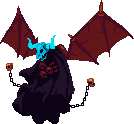
\includegraphics[width=\textwidth]{imagens/demon-idle.png}
    \end{minipage}
    \hfill
    \begin{minipage}[b]{0.25\textwidth}
        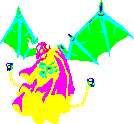
\includegraphics[width=\textwidth]{imagens/demon-idle.expected.png}
    \end{minipage}
    \hfill 
    \begin{minipage}[b]{0.25\textwidth}
        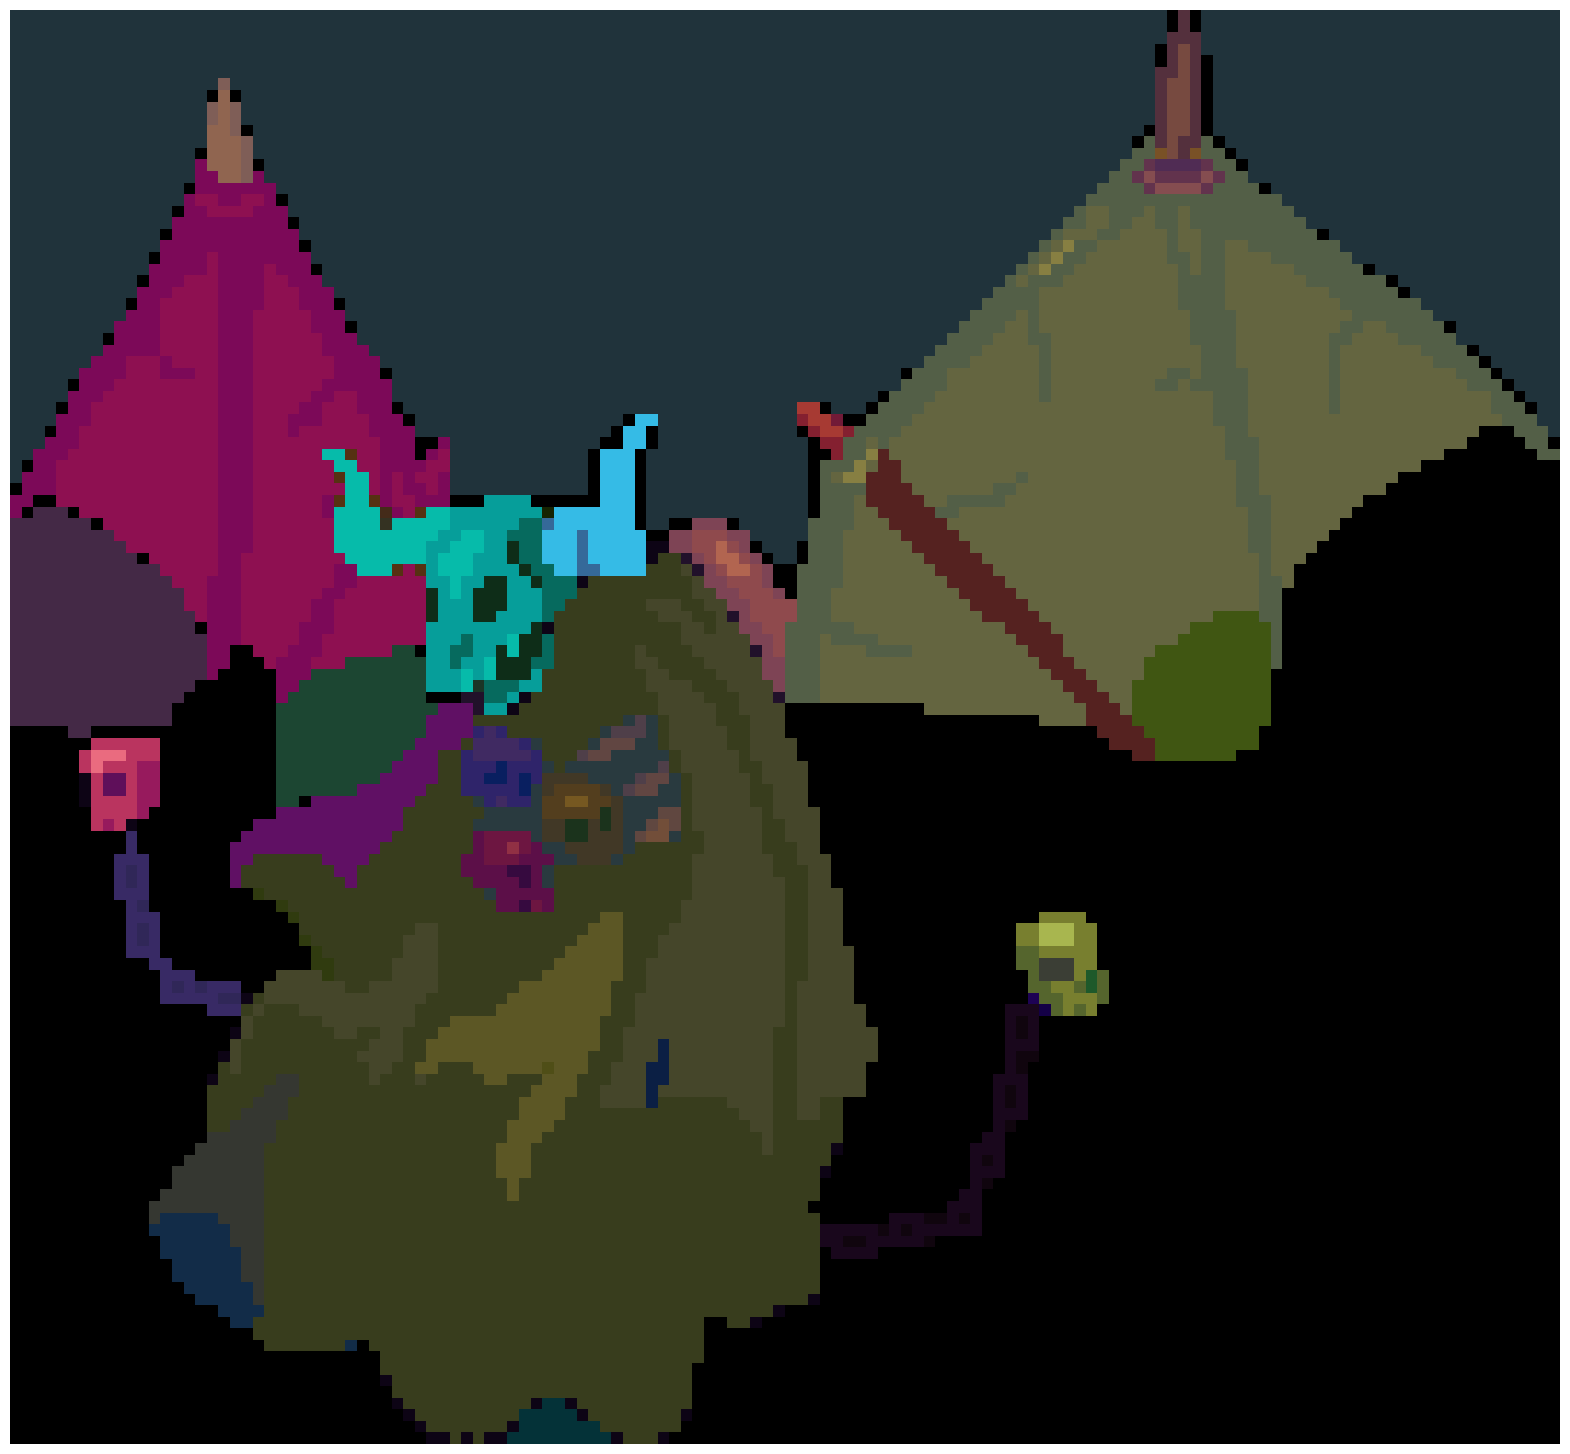
\includegraphics[width=\textwidth]{imagens/demon-idle.result.png}
    \end{minipage}
\end{figure}

\begin{figure}[h!]
	\caption{A imagem com o pior resultado (NCC)}
    \label{fig:badncc}
    \centering
    \begin{minipage}[b]{0.25\textwidth}
        
\includegraphics[width=\textwidth]{imagens/01_dish.png}
    \end{minipage}
    \hfill
    \begin{minipage}[b]{0.25\textwidth}
        
\includegraphics[width=\textwidth]{imagens/01_dish.expected.png}
    \end{minipage}
    \hfill 
    \begin{minipage}[b]{0.25\textwidth}
        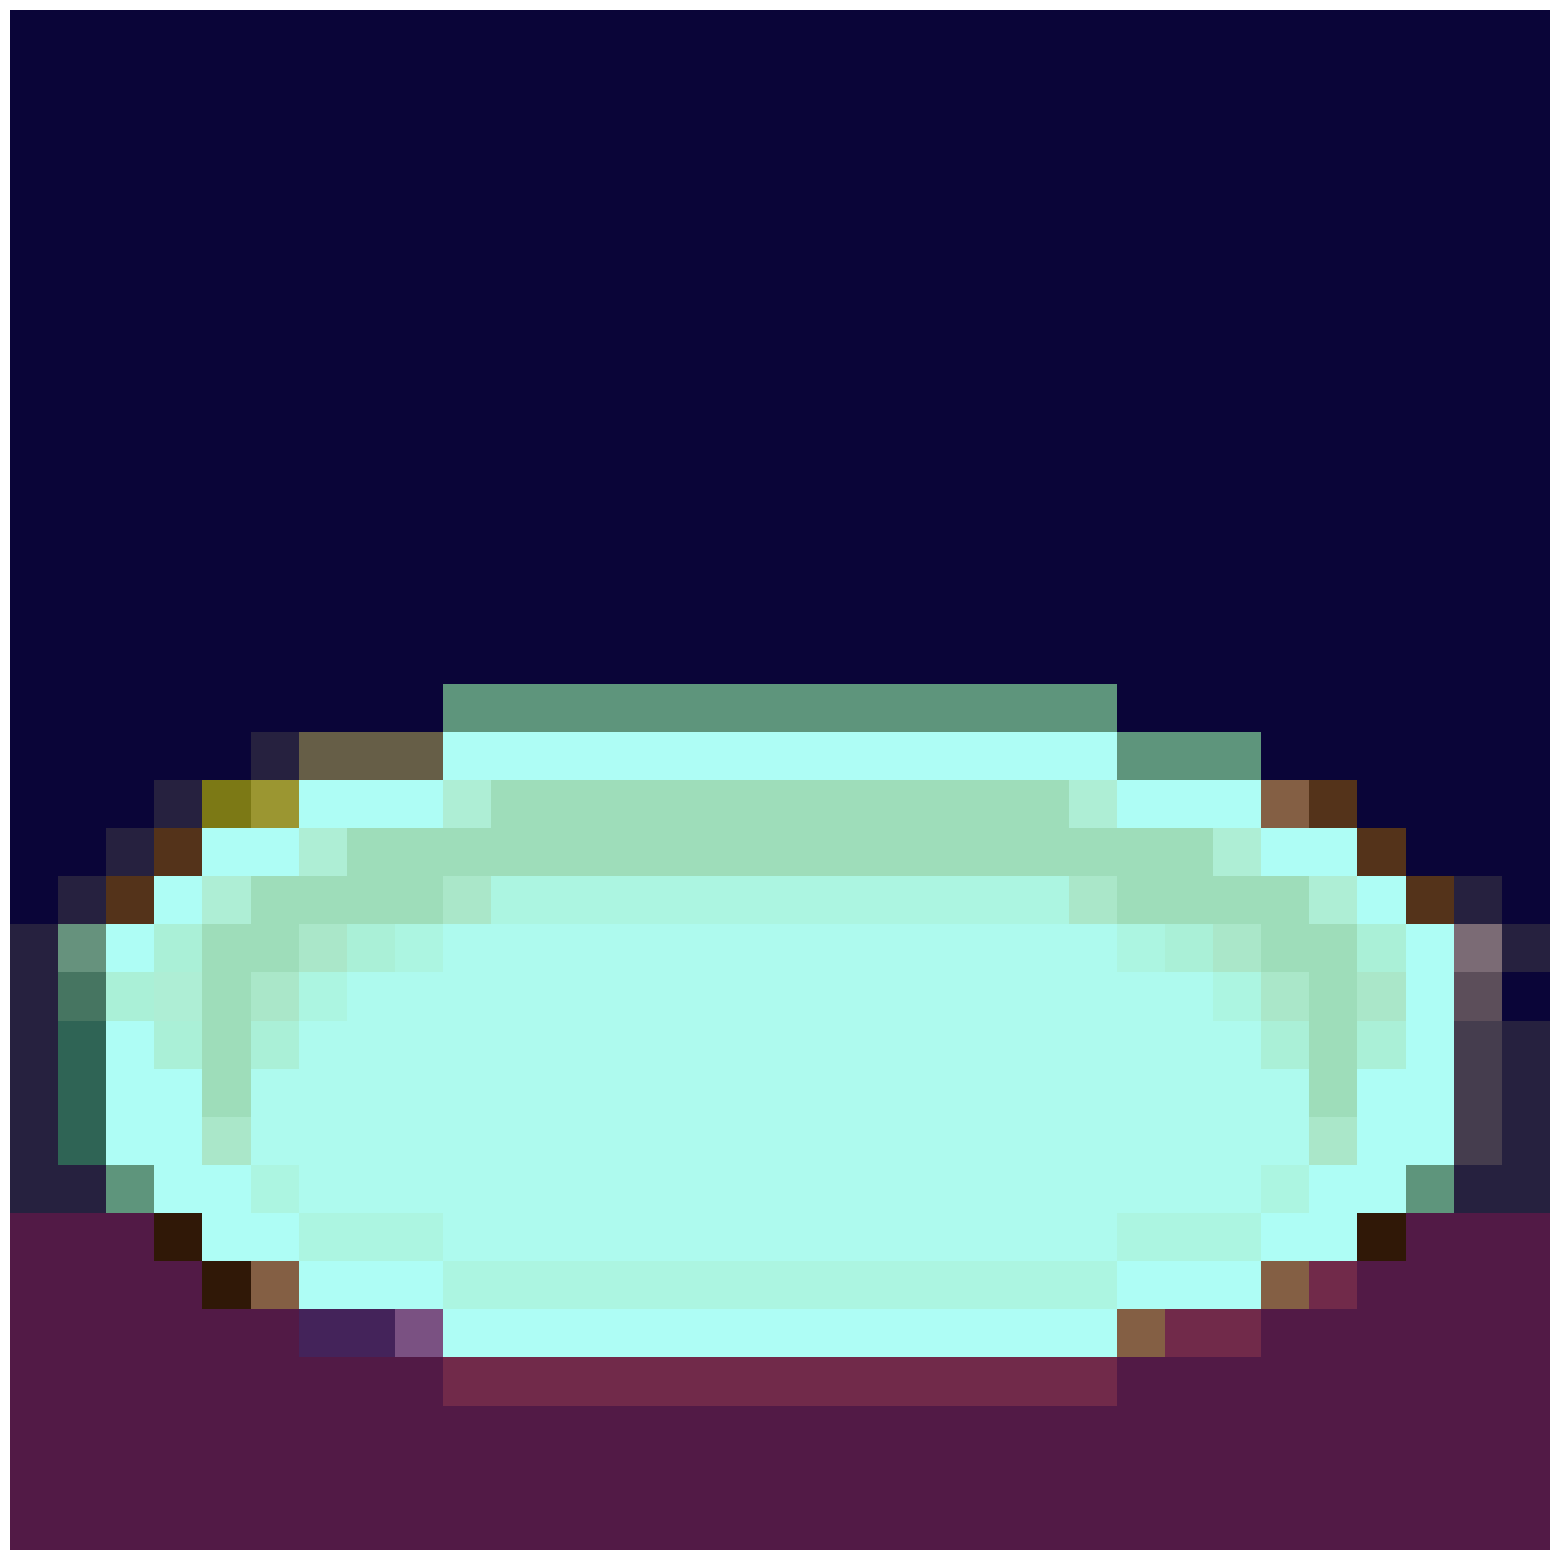
\includegraphics[width=\textwidth]{imagens/01_dish.result.png}
    \end{minipage}
\end{figure}

\begin{figure}[h!]
	\caption{A imagem com o melhor resultado (MSE)}
    \label{fig:bestmse}
    \centering
    \begin{minipage}[b]{0.25\textwidth}
        
\includegraphics[width=\textwidth]{imagens/nightmare-idle.png}
    \end{minipage}
    \hfill
    \begin{minipage}[b]{0.25\textwidth}
        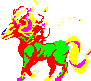
\includegraphics[width=\textwidth]{imagens/nightmare-idle-v2.png}
    \end{minipage}
    \hfill 
    \begin{minipage}[b]{0.25\textwidth}
        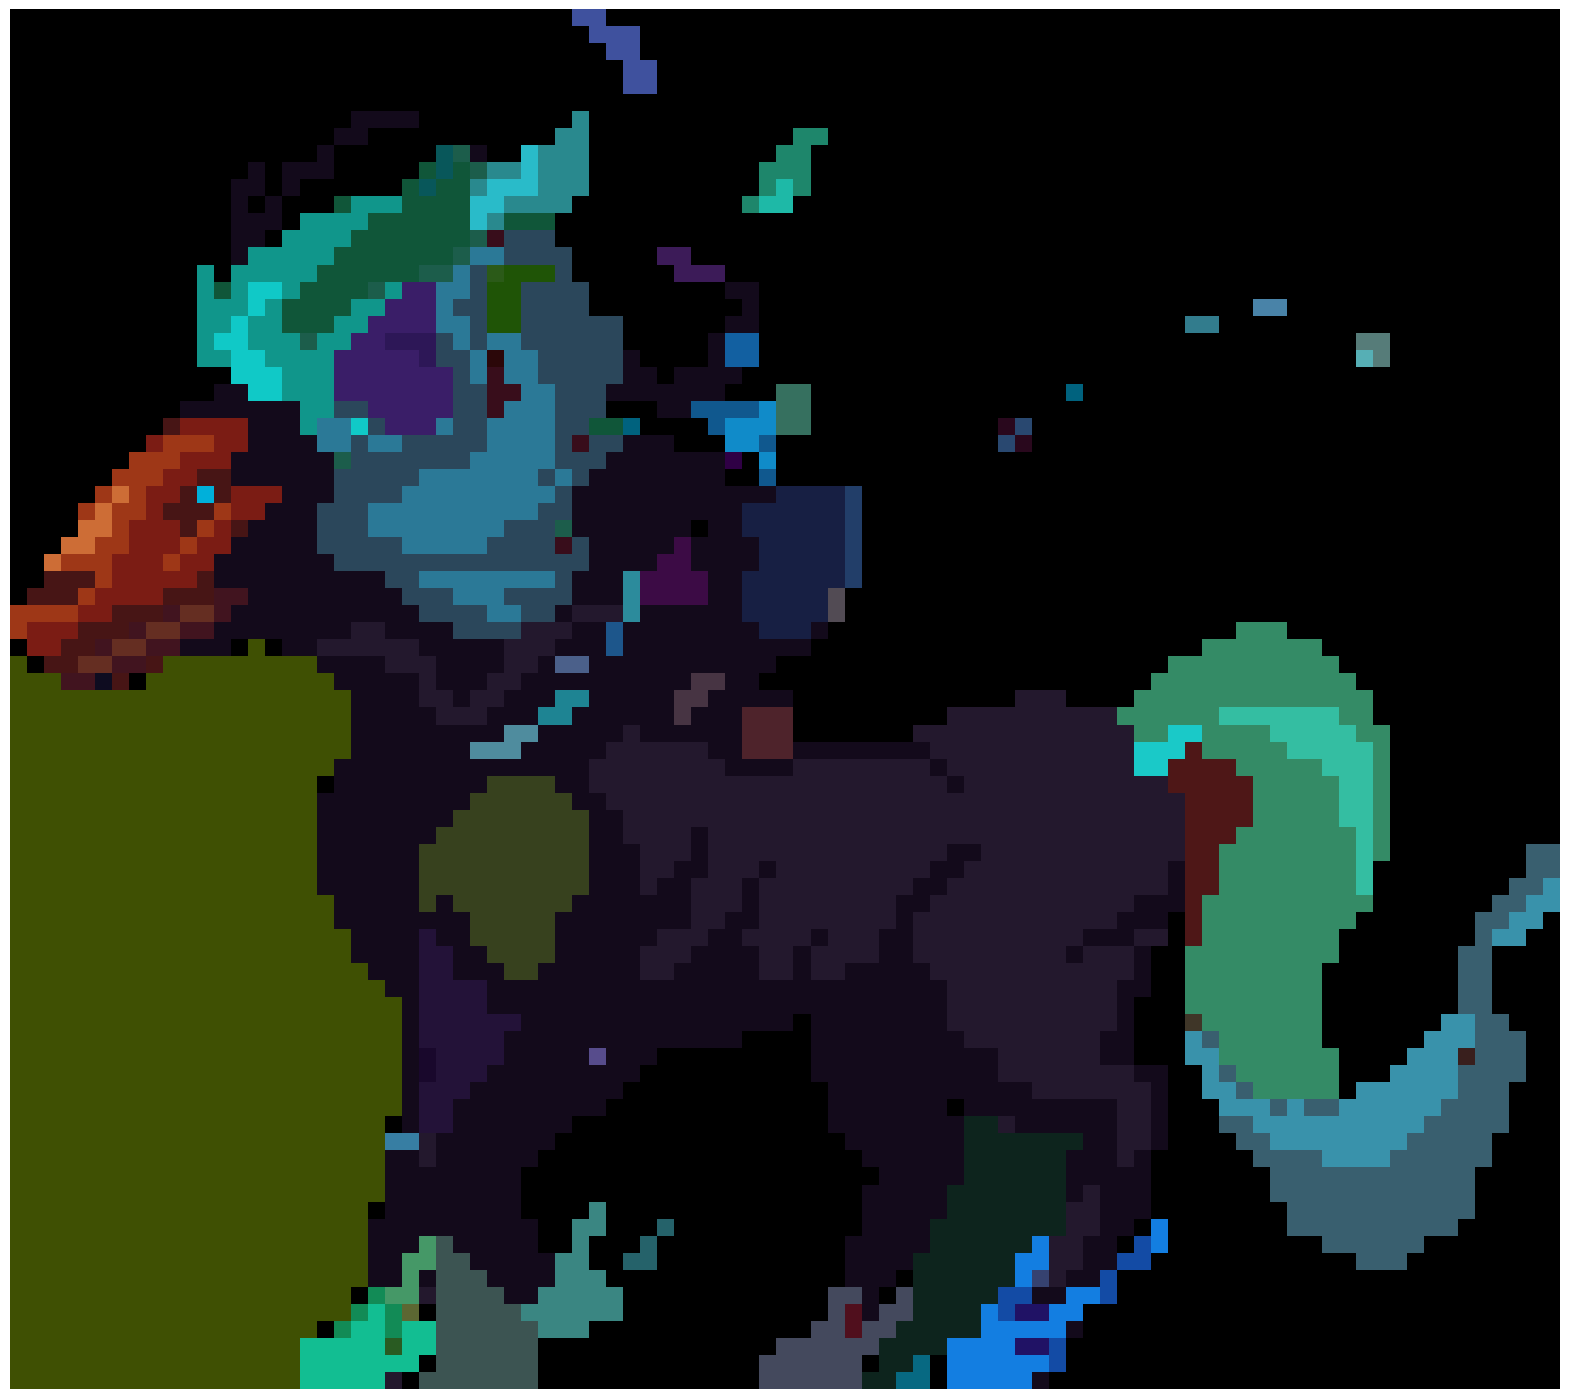
\includegraphics[width=\textwidth]{imagens/Result3.png}
    \end{minipage}
\end{figure}

\begin{figure}[h!]
	\caption{A imagem com o pior resultado (MSE)}
    \label{fig:badmse}
    \centering
    \begin{minipage}[b]{0.25\textwidth}
        
\includegraphics[width=\textwidth]{imagens/41_eggsalad_bowl.png}
    \end{minipage}
    \hfill
    \begin{minipage}[b]{0.25\textwidth}
        
\includegraphics[width=\textwidth]{imagens/41_eggsalad_bowl.expected.png}
    \end{minipage}
    \hfill 
    \begin{minipage}[b]{0.25\textwidth}
        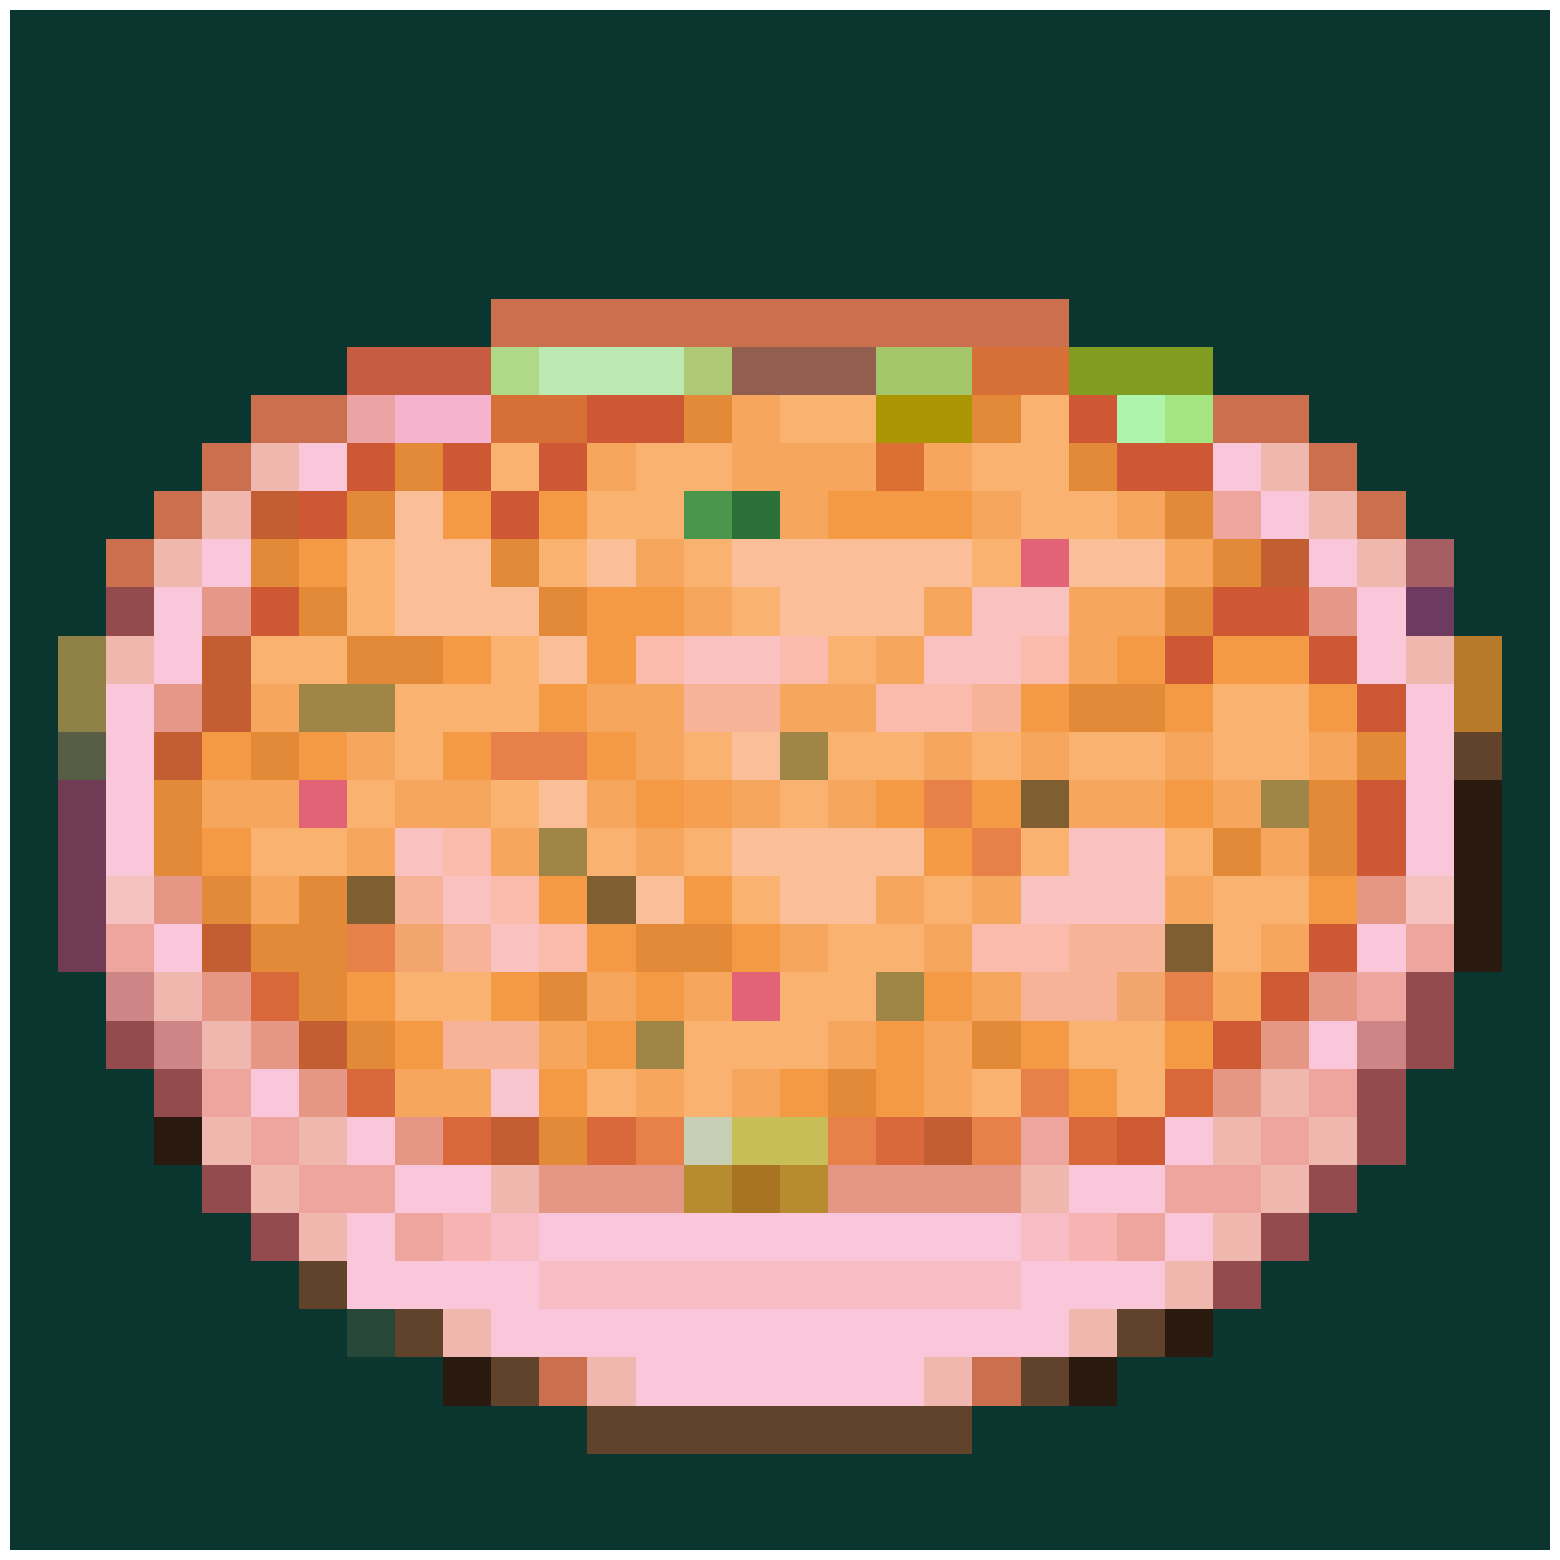
\includegraphics[width=\textwidth]{imagens/41_eggsalad_bowl.result.png}
    \end{minipage}
\end{figure}

Durante a análise dos resultados utilizando as métricas MSE e NCC, foi possível identificar algumas diferenças marcantes em seus comportamentos.

Considerando que as métricas assimilam como melhor resultado as figuras com menor taxa de erro e pior resultado as figuras que apresentam mais divergências da imagem original, percebe-se que no caso do MSE, os resultados não foram compatíveis com o esperado.

Na Figura \ref{fig:bestmse}, identificada como melhor resultado, não foram capturadas erros marcantes e aspectos importantes, como bordas e texturas, os quais são facilmente visualizados.

O mesmo acontece no pior resultado, pois a figura é próximo ao objeto original, mas a análise não conseguiu identificar tais similaridades, reforçando as limitações dessa métrica para análises perceptivas e estruturais seguindo o contexto das mascaras realizadas pelo (SAM).

Isso ocorre porque o MSE avalia diferenças absolutas entre os pixels, ignorando o contexto visual da imagem. 

Por outro lado, com o NCC, o cenário foi um pouco diferente. No melhor resultado, o NCC pareceu corresponder melhor à qualidade perceptiva da imagem, já que identifica a similaridade estrutural entre as imagens. Isso ficou evidente na imagem que apresenta altos níveis de segmentação, com contornos bem definidos e características mais preservadas. Comparado ao MSE, o NCC mostrou-se mais confiável para avaliar a relação entre as estruturas das imagens, especialmente em cenários onde a segmentação é um fator crítico.

De forma geral, essa análise reforça que o MSE, nem sempre reflete a qualidade perceptiva ou funcional dos resultados. Métricas como o NCC, que consideram a similaridade estrutural, podem ser mais adequadas para avaliar imagens segmentadas. Para melhorar a análise, que avalia similaridades perceptuais, e explorar ajustes no método utilizado para gerar as imagens, principalmente em cenários onde o MSE apresentou maior discrepância.
